
\chapter{Proposed Approach}
\thispagestyle{plain}



\label{Chapter3}

This chapter is about our proposed cybersecurity event extraction system. First the overview of the system are shown, followed by details of each components in the system, including tools that we planned to use in each steps for developing our system.

\section{System Architecture}
\label{architecture}
Our system architecture is shown in Figure \ref{fig:systemarch}. The system consists of annotation process and event extraction process. Each process will be described in the following section.

\begin{figure}
    \centering
    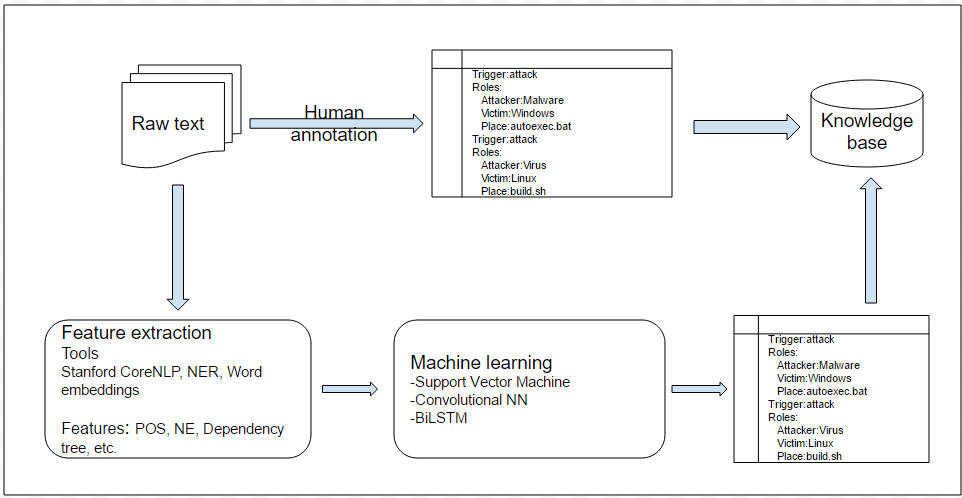
\includegraphics[width=\textwidth]{systemarch}
    \caption{System Architecture}
    \label{fig:systemarch}
\end{figure}

\section{Data Sources}
\label{datasources}
Our input/raw text will be in the unstructured form, most of them are chunks or pieces of text from the world wide web or discussion forums. These data sources are National Vulnerabilities Database (NVD), Microsoft Security Bulletins, collections of threats reported from antivirus software. The short description of each data sources will be given as follows:
\begin{itemize}
    \item National Vulnerabilities Database (NVD) is a government repository of standards-based vulnerability information.The NVD is a product of the National Institute of Standards and Technology (NIST) Computer Security Division. This data enables automation of vulnerability management, security measurement, and compliance. NVD includes databases of security checklists, security related software flaws, misconfigurations, product names, and impact metrics.
    \item Microsoft Security Bulletin is managed by the Microsoft Security Response Center. They releases security bulletins on a monthly basis addressing security vulnerabilities in Microsoft software, describing their remediation, and providing links to the applicable updates for affected software. 
\end{itemize}
Besides, some other sources may be included in the future if they are provided for expanding the knowledge base.

\section{Data Annotation}
\label{dataannotation}
We will design our event ontology by extending it from the UCO ontology \cite{syed2016uco}. The ontology will be sketch from the observed event information from the annotation event from our corpus. After we designed the event ontology for our cybersecurity data, the ontology will be used in the annotation process. The ontology will be in the form of slot filling. The annotation will be done by human who has strong background in cybersecurity. The annotators have to read through these raw text to find the interested event. Then they have to fill in the slot for each detected events. For example, \textit{"The malware A replicates the file a.jpg in the C system after user entered the foo website."} The event trigger \textit{"replicate"} has to be identified along with \textit{"C system"}, \textit{"a.jpg"} , and \textit{"malware A"}. \\
\indent For quality of annotating data, we will perform inter-annotator agreement checking for each event detected. Each event will be kept only when it is the majority vote event. When the annotation process is done, the ambiguity, consistency, and quality of annotation will be analyzed. The quality assessment process of data annotation will be explained in the Evaluation chapter (Chapter \ref{Chapter5}).

\section{Feature Extraction}
\label{featureextraction}
One of the crucial step in building information extraction system is the feature engineering. Good feature set can be represented for any instances of its class. We will experiment with features that were used in the event extraction researches in the past. Features are categorized into four classes described as follows:
\begin{itemize}
    

\item \textbf{Lexical features} include the word itself, its sub-units and its grammar function in the sentence. The Stanford CoreNLP \cite{manning2014stanford} will be used to find these lexical features. Features are:
\begin{enumerate}
    \item Unigram/bigram of the token
    \item Unigram/bigram of part-of-speech tags of the token
    \item Lemma of the token 

\end{enumerate}

\item \textbf{Syntactic features} are from the dependency parse tree. They will help the system to find the same functional word as the token in sentences. The Stanford CoreNLP \cite{manning2014stanford} will be used to build the dependency parse tree. These features consist of:
\begin{enumerate}
    \item Dependent and governor words of the token 
    \item Dependency types associated the token 
    \item Depth of node in its syntactic parse tree
    \item The path from the leaf node to the root node
    \item Part-of-speech of the child dependencies and head dependencies
    \item Head word of subject and object of the token

\end{enumerate}

\item \textbf{Semantic features} represent the basic conceptual components of meaning for any lexical item. They will help the system in expanding the possible token that has the same general meaning. Wordnet \cite{fellbaum1998wordnet} will be used to find synonyms, hypernyms. For word embeddings, there are still no pre-trained cybersecurity domain word embeddings in the market. We have to build the word embeddings for cybersecurity domain. We will follow context embeddings \cite{mikolov2013efficient} and dependency embeddings \cite{levy2014dependency}. The semantic features we will use in our system are:
\begin{enumerate}
    \item The first synset of the token from Wordnet
    \item Hypernym of the token, and its parent
    \item Context word embeddings of the token.
    \item Dependency word embeddings of the token. 
\end{enumerate}

\item \textbf{Entity features} are information about named entities appeared in the surrounding of the token. About entity features in our context we cannot use the Stanford CoreNLP, because the tool cannot recognize computer technical terms well. We will use the Cybersecurity Entities and Concept Spotter developed by \cite{lal2013} and improve its performance if necessary. Entity features consist of: 
\begin{enumerate}
    \item Nearest entity type in the sentence.
    \item Entity types of the subject of the token.
    \item Entity types of the object of the token.
    
\end{enumerate}

\end{itemize}

\section{Machine Learning}
\label{machinelearning}
We will solve the event extraction problem based on the idea that same event class/type always appears in the same context. We can classify the input to our event class using the classification algorithm. After we extracted features, we need algorithm to classify features into pattern or class as output. We introduced three methods to be experiment with our features. There are Support Vector Machine, Convolutional Neural Network, and Bidirectional Long Short Term Memory. Each algorithm will be explained as follows.

\subsection{Support Vector Machine}
Support Vector Machine (SVM) is a supervised machine learning algorithm which can be used for both classification or regression analysis. However,  it is mostly used in classification problems. Given a set of labeled training examples, each marked as belonging to one or the other of two categories, an SVM training algorithm builds a model that assigns new examples to one category or the other, making it a non-probabilistic binary linear classifier. In this algorithm, we plot each data item as a point in n-dimensional space where n is number of output classes with the value of each feature being the value of a particular coordinate. Then, we perform classification by finding the hyperplane that differentiate these classes very well. Figure \ref{fig:svm} shows the hyperplane that separate features into two classes.
\begin{figure}
    \centering
    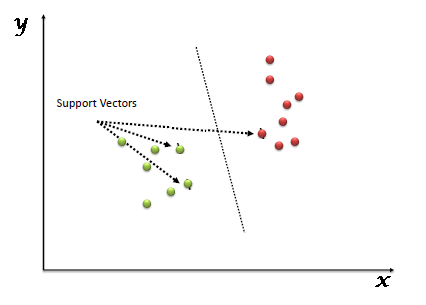
\includegraphics{svm}
    \caption{Support Vector Machine hyperplane}
    \label{fig:svm}
\end{figure}
Support vector machine was introduced in many natural language processing researches. For example,  \cite{satyapanich2015ebiquity} used support vector machine to classify features for measuring semantic similarity between twitters data. \cite{kashyap2016robust} in word2sense part, support vector machine was used for predicting the semantic similarity between word and its sense. Moreover, support vector machine have also been used in Event Extraction research. \cite{tsetsai2016event} use support vector machine with L2 regularization loss to classify features (such as lexical features, features from parser, Named Entity Recognition (NER), Semantic Role Labeling (SRL), entity co-reference ) to detect TAC 2016 event mention and \cite{satyapanich2016event} used support vector machine in classify features (such as frequency of each name entity types, part of speech) to predict TAC 2016 event triggers.  \\
\indent In our work, we will use support vector machine to classify features into event classes by using the WEKA tools \cite{hall2009weka}. Weka is a collection of machine learning algorithms for data mining tasks.  Weka contains tools for data pre-processing, classification, regression, clustering, association rules, and visualization. It also comes with packages to help in facilitate in experiments such as AutoWeka \cite{thornton2013auto}. Autoweka is a plugin that automatically selects a learning algorithm, set its hyperparameters and gives the accuracy of each settings. User set only one running time parameter. 

\subsection{Convolutional Neural Network}
Convolutional neural network is a type of feed-forward artificial neural network. CNNs are basically several layers of convolutions with nonlinear activation functions like tanh applied to the results. The main difference from other neural networks is to use convolutions over the input layer. This results in connection to the next layer where the input data are grouped into regions and  connect to a neuron in the output. Each layer applies different filters and combines their results. 
The input to most natural language processing tasks are sentences or documents represented as a matrix. Each row of the matrix corresponds to one token or word. That is, each row is vector that represents a word. Typically, these vectors are word embeddings like word2vec or GloVe. For a 5 words sentence using a 50-dimensional embedding we would have a 5×50 matrix as our input. An example of CNN applied with natural language processing task is in Figure \ref{fig:convnn}.
\begin{figure}
    \centering
    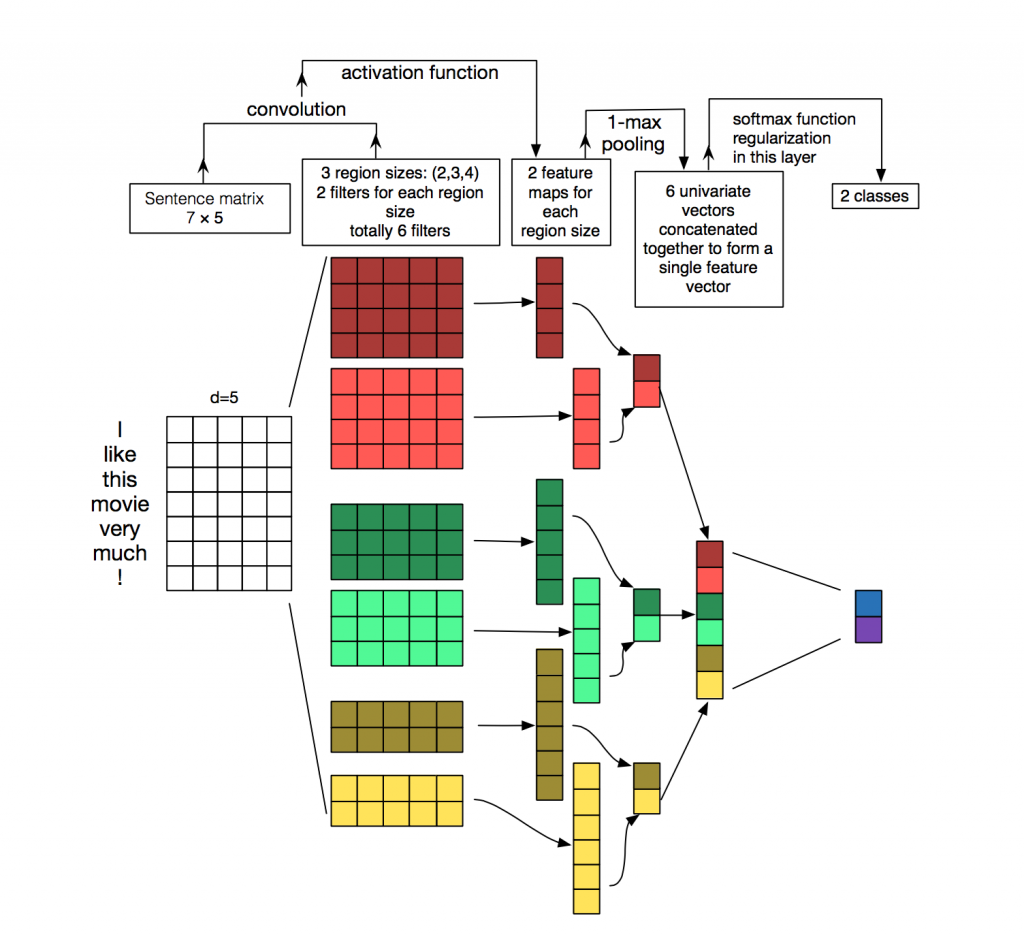
\includegraphics[width=\textwidth]{convnn}
    \caption{Convolutional Neural Network applied with NLP. Source: (Zhang and Wallace 2015)}
    \label{fig:convnn}    
\end{figure}\\
\indent There are several natural language processing research applied CNN in classification task. For example, \cite{kim2014convolutional} used CNN to sentiment classification in sentence level. The input layer is a sentence composed from concatenated word2vec word embeddings. A convolutional layer with multiple filters, fully connects to a max-pooling layer, and finally a softmax classifier. A similar neural network architecture was previously proposed in \cite{kalchbrenner2014convolutional}. \cite{zhang2015sensitivity} performs an empirical evaluation on the effect of varying hyperparameters in CNN architectures, investigating their impact on performance and variance over multiple runs. \cite{nguyen2015relation} explores CNNs for  Relation Extraction and Relation Classification tasks. In addition to the word vectors, the authors use the relative positions of words to the entities of interest as an input to the convolutional layer. This models assumes that the positions of the entities are given, and that each example input contains one relation.\\
\indent We will extend our work \cite{satyapanich2016event} for event nugget detection. This work was implemented by Tensorflow \cite{tensorflow2015-whitepaper}. It functioned as sentence classification. It classify the input sentence to be one class of event. But it used only word embeddings as feature. We will improve its performance by adding features mentioned in the previous section.

\subsection{Bidirectional Long Short Term Memory Neural Networks}
\label{bilstm}
Bidirectional Long Short Term Memory Neural Networks (BiLSTMs) are a sophisticated form of Recurrent Neural Network. Traditional Recurrent Neural Networks (RNNs) perform the same task for every element of a sequence, with the output being depended on the previous computations. RNNs have a memory which captures information about what has been calculated so far. In theory RNNs can make use of information in arbitrarily long sequences, but in practice they are limited to looking back only a few steps. \cite{Hochreiter:1997:LSM} introduced Long Short Term Memory to store information over extended time intervals, which are much better at capturing long-term dependencies than RNNs are. LSTMs have the same architecture as RNNs, but they use a different function to compute the hidden state. Figure \ref{fig:lstm} shows diagram of a LSTM cell. \\
\begin{figure}
    \centering
    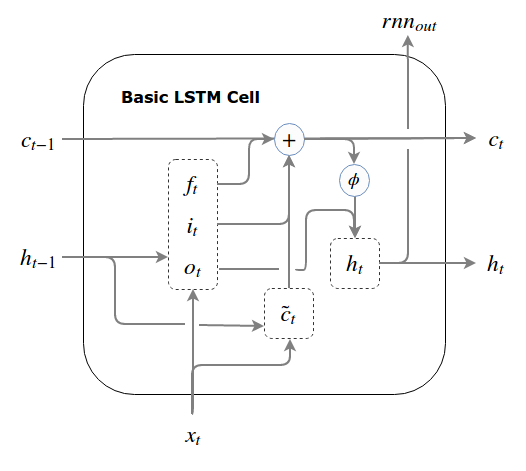
\includegraphics[width=0.5\textwidth]{lstm}
    \caption{A LSTM cell}
    \label{fig:lstm}
\end{figure}
\indent Internally these cells in the LSTMs make the decision what to keep or what to forget follows equation 3.1-3.5. These equations are computed using the previous state, the current memory, and the input. \\
\begin{equation}
    f_t=\sigma_g(W_f x_t + U_f h_{t-1} + b_f)
\end{equation}
\begin{equation}    
    i_t=\sigma_g(W_i x_t + U_i h_{t+1} + b_i)
\end{equation}
\begin{equation}
    o_t=\sigma_g(W_o x_t + U_o h_{t-1} + b_o)    
\end{equation}
\begin{equation}
    c_t=f_t \circ c_{t-1} + i_t \circ \sigma_c(W_c x_t + U_c h_{t-1} + b_c)
\end{equation}
\begin{equation}
    h_t=o_t \circ \sigma_h(c_t)
\end{equation}
where 
\begin{itemize}
\item $x_t$ is input vector.
\item $h_t$ is output vector.
\item $c_t$ is cell state vector.
\item $W , U$ and $b$ is parameter matrices and vector.
\item $f_t$ is forget gate vector, weight of keeping old information.
\item $i_t$ is input gate vector, weight of acquiring new information.
\item $o_t$ is output gate vector.
\item $\sigma$ is an activation function.
\end{itemize}
\indent Bidirectional RNNs are focused on the direction of transition of Neural Network state. It based on the idea that the output at time t may not only depend on the previous elements in the sequence, but also future elements. For example, to predict a token in a sentence you want to look at both the left and the right context. Bidirectional RNNs are just two RNNs stacked on top of each other as showed in Figure \ref{fig:birnn}. The output is then computed based on the hidden state of both RNNs.\\
\begin{figure}
    \centering
    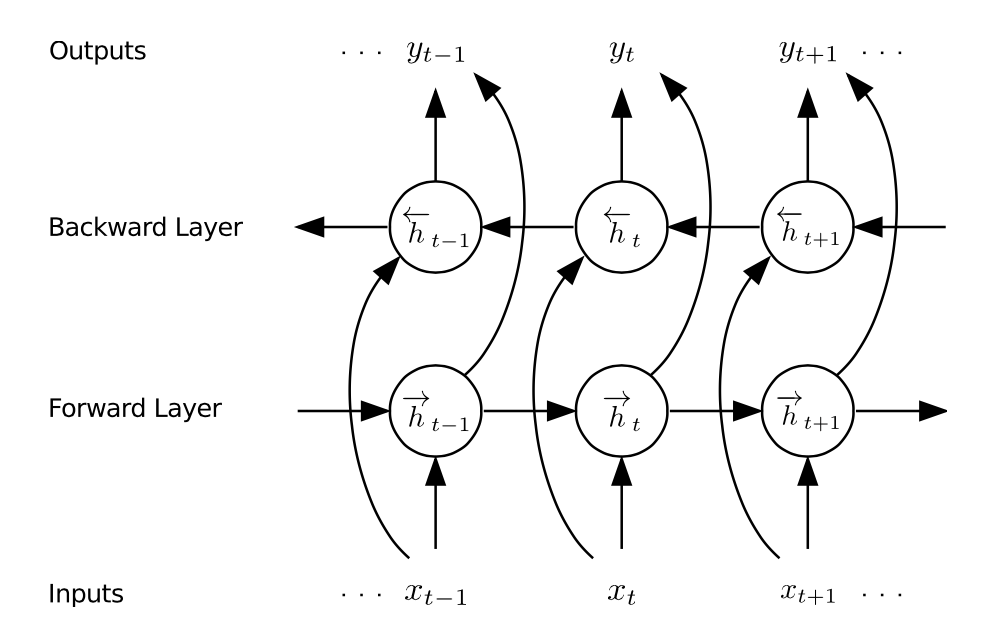
\includegraphics[width=0.6\textwidth]{birnn}
    \caption{Bidirectional Recurrent Neural Network}
    \label{fig:birnn}
\end{figure}
\indent Bidirectional LSTMs have the same architecture as Bidirectional RNNs but use LSTM for each state instead of RNN. BiLSTMs are two LSTMs that computed in different direction. They are used in many natural language processing research recently. In TAC 2016 shared tasks event track, there are some participants used BiLSTM to detect events. They showed good performance in event mention detection task. For example, \cite{zeng2016event}  trained a LSTM neural network model that labels each sentence in the BIO scheme. Specifically, a word is labeled as B if it is he beginning of a trigger of type ,or I if it is inside a trigger of type, or O otherwise.  They used 100 LSTM hidden states. \cite{mihaylov2016event} also used LSTMs to encode the event trigger in the sentence tokens with average word embeddings features. We will implement BiLSTMs using Tensorflow.